\chapter{Oprogramowanie}

Oprogramowanie całej konstrukcji składa się z 2 części, są to:
\begin{itemize}
    \item program mikrokontrolera STM,
    \item program minikomputera Raspberry Pi.
\end{itemize}
Oba programy komunikują się ze sobą przez magistralę UART.

\section{Miktrokontroler STM}
Mikrokontroler został zaprogramowany z wykorzystaniem narzędzie \textit{STM32CubeIDE} \cite{cudeide}, które udostępnia producent układu. Środowisko pozwala w sposób graficzny na skonfigurowanie całego mikrokontrolera. Program został napisany w języku C z wykorzystaniem biblioteki \textit{Hardware Abstraction Layer -- HAL}. Konfiguracja wejść i wyjść mikrokontrolera przedstawiona jest na rysunku \ref{fig:stmconfig}.\\
W celu uniknięcia sytuacji potencjalnie niebezpiecznych mogących doprowadzić do zniszczenia komponentów zaprogramowano zabezpieczenia, które mają najwyższy priorytet w sytuacji krytycznej. Przewidziane sytuacje niebezpieczne to
\begin{itemize}
    \item dojechanie do końca profilu,
    \item uderzenie z dużą prędkością.
\end{itemize}

\subsection{Zabezpieczenia}
\subsubsection{Dozwolony zakres ruchu}
W celu przeciwdziałania uszkodzenia sterownika silnika i samego silnika dozwolony zakres ruchu wózka został ograniczony przez czujniki krańcowe założone na obu końcach profilu, po którym porusza się wózek. Funkcja reaguje na zbocze opadające sygnału z czujników. W przypadku wykrycia zmiany sygnału ze stanu wysokiego na niski, funkcja przerywa działanie programu ustawiając flagę końca programu na wartość 1. Wiąże się to z zatrzymaniem działania algorytmu oraz sterowania silnikiem, a na płytce deweloperskiej STM32F4Discovery zaczyna migać czerwona dioda sygnalizująca przerwanie programu. 

\subsubsection{Zwalnianie przy położeniach krańcowych}
W celu uniknięcia uderzeń w ograniczniki ruchu wózka funkcja odpowiedzialna za sterowanie silnikiem została zaprojektowana tak, aby nie doprowadzać do takiej sytuacji. Funkcja monitoruje położenie wózka na osi X. Jeżeli wózek jest w odległości mniejszej niż 10mm od granicy ruchu sterownik przechodzi w tryb hamowania, tak aby wózek nie uderzył w ogranicznik ruchu.

\section{Obsługa enkoderów}
W konstrukcji zostały wykorzystane 2 enkodery inkrementalne. Dzięki nim mikrokontroler jest w stanie obliczyć kąt odchylenia wahadła oraz pozycję wózka na osi X. Do obsługi czujników obrotu został wykorzystany tryb wejścia \textit{Encoder Mode}, który jest dedykowanym rozwiązaniem. Tryb pozwala zdefiniować czy impulsy są liczone z abu kanałów czy z jednego. Ponadto można zdefiniowac czy liczone są zbocza zarówno rosące jak i opadające, czy jedne z nich. Dodatkowo tryb \textit{Encoder Mode} ma wbudowny filtr, którego pozom działania ustawia się od 0 do 15. Testy wykazały, że zastosowania wbudowanego filtra jest wystarczajace. W odczytywanych sygnałach nie pojawiał się szum, odczyty były dokładne, woboc czego nie było potrzeby stosowania dodatkowego filtru sprzętowego lub programowego. 


\section{Raspberry Pi}
Na minikomputerze Raspberry Pi został zainstalowany dedykowany system \textit{Raspberry Pi OS} \cite{raspbian}. Jest to system z rodziny Linux, oparty na dystrybucji Debian. Obraz instalacyjny systemu zawiera wszystkie potrzebne sterowniki, które pozwalają na wykorzystanie wszystkich peryferiów minikomputera.\\
Aplikacja, która wyświetla i pozwala edytować ustawienia została stworzona w środowisku \textit{Node-Red} \cite{nodered}, która pozwala w sposób graficzny na zbudowanie funkcjonalnego programu. Środowisko to korzysta z języka \textit{JavaScript}, a budowanie programu polega na łączenie ze sobą odpowiednich bloczków. Każdy blok można odpowiednio skonfigurować, a możliwości całego środowiska rozszerza bogata biblioteka wtyczek. Istnieje również możliwość stworzenia własnego bloku programu, w którym mieści się kod w języku \textit{JavaScript}. Programowanie w środowisku \textit{Node-Red} standardowo dostępne jest na porcie 1880 komputera, na którym się znajduje i korzysta się z niego przez przeglądarkę internetową. Aplikacja zademonstrowana jest na rysnku \ref{fig:nodered}.

\begin{figure}
    \centering
    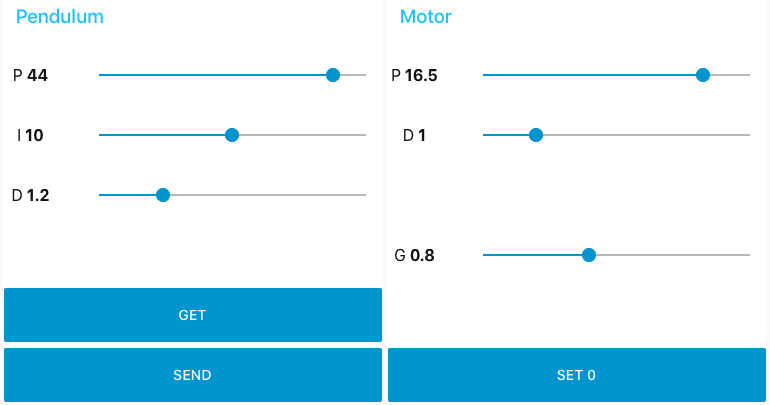
\includegraphics[width=\textwidth]{praca_dyplomowa/figures/nodered.png}
    \caption{Wygląd aplikacji umożliwiającej zmianę nastaw regulatorów}
    \label{fig:nodered}
\end{figure}

\section{Komunikacja}
Jako formę komunikacji pomiędzy urządzeniami wybrano protokół transmisji szeregowej UART. Wybór protokółu komunikacji wynika z bezproblemowej i łatwej implementacji w obu urządzeniach. Ponadto, do komunikowania się mikrokontrolera i komputera nie jest wymagana duża szybkość przesyłu. Protokół UART został skonfigurowany w następujący sposób na obu urządzeniach:
\begin{itemize}
    \item szybkość transmisji 115200 Bps
    \item 8 bitów
    \item 0 bitów parzystości
\end{itemize}

Komunikacja pomiędzy urządzeniami wykorzystana jest do edycji współczynników wpływających na regulację wahadła. Na ekranie dostępne są suwaki, które odpowiedzialne są za współczynniki algorytmu sterowania. Oprócz tego widoczne sa 3 przyciski:
\begin{itemize}
    \item \textit{SEND} -- wysyła nowe ustawienia,
    \item \textit{GET} -- pobiera aktualne ustawienia,
    \item \textit{SET 0} -- resetuje pomiar wychylenia wahadła.
\end{itemize}
Opcja \textit{Send} wysyła nowe współczynniki całego algorytmu w postaci ramki danych: \[H\,pp\,pi\,pd\,mp\,md\,wsp\]
gdzie:
\begin{itemize}
    \item \textit{H} -- nagłówek wiadomości,
    \item \textit{pp} -- nastawa członu proporcjonalnego regulatora wahadła, 
    \item \textit{pi} -- nastawa członu całkującego regulatora wahadła,
    \item \textit{pd} -- nastawa członu różniczkującego regulatora wahadła,
    \item \textit{mp} -- nastawa członu proporcjonalnego regulatora położenia,
    \item \textit{md} -- nastawa członu różniczkującego regulatora położenia,
    \item \textit{wsp} -- stosunek regulatora położenia do regulatora wahadła.
    \label{it:ramka}
\end{itemize}
Nagłówek wiadomości to informacja dla mikrokontrolera, który przycisk został naciśnięty:
\begin{itemize}
    \item \textit{P -- Send} -- zmienia współczynniki algorytmu na te przesłane w wiadomości,
    \item \textit{G -- Get} --  wysyła aktualne ustawienia,
    \item \textit{S -- Set 0} -- resetuje pomiar wychylenia wahadła.
\end{itemize}
W odpowiedzi na każdą nadesłaną wiadomość mikrokontroler odsyła do Raspberry Pi ramkę danych w postaci pliku JSON ("klucz":wartość):
\[\{"pp":44.00,"pi":10.00,"pd":1.20,"mp":16.50,"md":1.00,"wsp":0.80\}\] 
gdzie:
\begin{itemize}
    \item \textit{pp} -- nastawa członu proporcjonalnego regulatora wahadła, 
    \item \textit{pi} -- nastawa członu całkującego regulatora wahadła,
    \item \textit{pd} -- nastawa członu różniczkującego regulatora wahadła,
    \item \textit{mp} -- nastawa członu proporcjonalnego regulatora położenia,
    \item \textit{md} -- nastawa członu różniczkującego regulatora położenia,
    \item \textit{wsp} -- stosunek regulatora położenia do regulatora wahadła.
    \label{it:ramka}
\end{itemize}

Mikrokontroler po otrzymaniu danych i sprawdzeniu ich poprawności wczytuje je jako aktualne ustawienia. 

